\oldpage{402}

With this treatment the patients all recovered after a longer or shorter
period.

\textsc{Note.---}The formula for preparing the acetic tincture of iron is to be
found on page 351 of the \ThisJournal{College Journal}.

\begin{figure}[H]
  \centering
  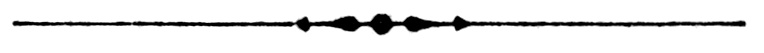
\includegraphics{pages/illustrations/arrow_bullet_divider.jpg}
\end{figure}

\section*{Pleuritis, Latant.}

\byline*{\ProperName{C.~E.\ Witham},\ \md}

\SectionStartWords{Pleuritis} is a disease which often presents obscure, important and interesting
complications, taxing the utmost skill of the experienced physician
in tracing the precise bearing and extent of the morbid action
established.

The heart, lungs, bronchia and liver are often implicated in this disease.
Asthenic pneumonia, and chronic and latent pleuritis have many common
symptoms. It is stated that pleuritis is more prone to produce
tubercular disease than pneumonia is, and it is thought by some authors
that the absorption of pus into the blood may explain this rather singular
fact. In the treatment of disease our object should be to remove
morbid action by the most simple and effectual treatment the case will
admit of. If the following report should be the means of stimulating
the young practitioner to a more thorough study of thoracic diseases I
shall be amply rewarded.

On the 11th of June, 1856, F.~W., a lad 14 years of age was presented
for my advice. He was of a sanguine temperament, and a twin brother.
I had never seen him before, but from his father gained the following
history of his case. Five months previous to calling upon me he suddenly
lost the power of speech; did not know that he had previously
suffered from cold or exposure. The loss of speech was the first symptom
of disease he could recollect and this was not preceded by any
very marked indications of hoarseness. A low, hoarse and painful
whisper was the result of all his efforts at conversation. This condition
continued for one month when to his surprise and great joy he found
himself complete master of his vocal organs and congratulated himself
on so strange and unexpected a recovery. He said that while making
some slight exertion he felt something give away in his chest and immediately
he could talk as well as ever. At the end of one week he
was again deprived of speech in the same unexpected and sudden manner.
His physician after inspecting his throat, but making no other
examination, prescribed a gargle of ``pepper tea'' saying it would soon\endinput
